\documentclass{beamer}
% Use lualatex to process this file
\usepackage{svg}
\usepackage[ngerman]{babel}
\usepackage{amsmath,amscd}
\usetheme{Hannover}
\title{Elliptische Kurven: Was ist das?}
\subtitle{Und wie macht man damit Kryptographie?}
\author{Nils Rennebarth}
\date{November 2024}
\newcommand{\C}{\mathbb{C}}
\newcommand{\F}{\mathbb{F}}
\newcommand{\N}{\mathbb{N}}
\newcommand{\Proj}{\mathbb{P}}
\newcommand{\Q}{\mathbb{Q}}
\newcommand{\R}{\mathbb{R}}
\newcommand{\Z}{\mathbb{Z}}
\newtheorem{folgerung}[theorem]{Folgerung}
\newtheorem{beispiel}[theorem]{Beispiel}
\begin{document}

% ----------------------
\begin{frame}
  \titlepage
\end{frame}
% ----------------------

\section{Einführung}
\begin{frame}
  \frametitle{Vorschau}
  \begin{itemize}
  \item Was sind elliptische Kurven und wie sehen sie aus?
  \item Addition von Punkten: geometrisch $\Longrightarrow$ arithmetisch.
  \item Übergang zur projektiven Ebene
  \item Wie rechnen Computer auf so etwas?
  \item Wie nutzt man das alles zur Kryptographie?
  \end{itemize}
\end{frame}

\begin{frame}
  \frametitle{Was sind elliptische Kurven}
  \framesubtitle<1-4>{Beispiel}
  \framesubtitle<5>{Dies ist \emph{keine} elliptische Kurve}
  \begin{figure}
  \includegraphics<1>[height=0.7\textwidth]{ec1-m2-p2.png}
  \includegraphics<2>[height=0.7\textwidth]{ec2-m2-p1.png}
  \includegraphics<3>[height=0.7\textwidth]{ec3-p1-p0.png}
  \includegraphics<4>[height=0.7\textwidth]{ec4-p0-p4.png}
  \includegraphics<5>[height=0.7\textwidth]{nec-m3-p2.png}
  \end{figure}
\end{frame}

\begin{frame}
  \frametitle{Was haben die mit Ellipsen zu tun?}
  \begin{itemize}
  \item Die Berechnung der Bogenlänge einer Ellipse führt auf Integrale die
    sich nicht in geschlossener Form lösen lassen.
  \item Die Umkehrfunktion davon kann man in die komplexen Zahlen hinein
    fortsetzen. Nennt man elliptische Funktionen.
  \item Mit so einer Funktion und ihrer Ableitung kann man eine 1-1 Abbildung
    von den Punkten einer elliptischen Kurve auf ein Parallelogramm der
    komplexen Ebene konstruieren.
  \item \dots{} also eher entferntere Verwandtschaft.
  \end{itemize}
\end{frame}

\begin{frame}
  \frametitle{Normalform}
  Allgemeine Kubik:

  \begin{equation*}
    a y^3 + b y^2 x + c y x^2 + d x^3 + e y^2 + f x y + g x^2 +
    h x + i y + j = 0
  \end{equation*}

  Es reicht jedoch, Kurven der folgenden Form zu betrachten:

  \pause
  \begin{definition}[Weißerstraß Normalform]
    Die Normalform einer elliptischen Kurve E über den reellen Zahlen
    $\R$ ist:

    \begin{equation}
      y^2 = x^3 + ax + b
      \label{eq:weier}
    \end{equation}

    mit a und b aus $\R$, wobei:
    \begin{equation}
      \Delta_E = -4a^3 - 27b^2 \ne 0
    \end{equation}
  \end{definition}
\end{frame}

% ----------------------

\section{Addition von Punkten}

\begin{frame}
  \frametitle{Addition von Punkten, geometrisch}
  \begin{figure}
    \includegraphics[height=0.7\textwidth]{ec5-m1-p1-add.png}
  \end{figure}
\end{frame}

\begin{frame}
  \frametitle{Addition von Punkten, mehrfach}
  \includegraphics<1>[height=0.7\textwidth]{ec7-addpt-000.png}
  \includegraphics<2>[height=0.7\textwidth]{ec7-addpt-001.png}
  \includegraphics<3>[height=0.7\textwidth]{ec7-addpt-002.png}
  \includegraphics<4>[height=0.7\textwidth]{ec7-addpt-003.png}
  \includegraphics<5>[height=0.7\textwidth]{ec7-addpt-004.png}
  \includegraphics<6>[height=0.7\textwidth]{ec7-addpt-005.png}
  \includegraphics<7>[height=0.7\textwidth]{ec7-addpt-006.png}
  \includegraphics<8>[height=0.7\textwidth]{ec7-addpt-007.png}
  \includegraphics<9>[height=0.7\textwidth]{ec7-addpt-008.png}
  \includegraphics<10>[height=0.7\textwidth]{ec7-addpt-009.png}
  \includegraphics<11>[height=0.7\textwidth]{ec7-addpt-010.png}
  \includegraphics<12>[height=0.7\textwidth]{ec7-addpt-011.png}
  \includegraphics<13>[height=0.7\textwidth]{ec7-addpt-012.png}
  \includegraphics<14>[height=0.7\textwidth]{ec7-addpt-013.png}
  \includegraphics<15>[height=0.7\textwidth]{ec7-addpt-014.png}
  \includegraphics<16>[height=0.7\textwidth]{ec7-addpt-015.png}
  \includegraphics<17>[height=0.7\textwidth]{ec7-addpt-016.png}
  \includegraphics<18>[height=0.7\textwidth]{ec7-addpt-017.png}
  \includegraphics<19>[height=0.7\textwidth]{ec7-addpt-018.png}
  \includegraphics<20>[height=0.7\textwidth]{ec7-addpt-019.png}
  \includegraphics<21>[height=0.7\textwidth]{ec7-addpt-020.png}
\end{frame}

\begin{frame}
  \frametitle{Addition, arithmetisch}
  \begin{theorem}[Additionsformel]
    Seien $P = (x_p, y_p)$ und $Q=(x_q, y_q)$ zwei Punkte auf der elliptischen
    Kurve $E$. Sei weiterhin:
    \begin{equation*}
      s = \left\{
        \begin{array}{l}
          \frac{y_p - y_q}{x_p - x_q} \text{ falls } x_p \ne x_q \\
          \\
          \frac{3x_p^2 + a}{2y_p}     \text{ falls } x_p = x_q, y_p \ne 0
        \end{array}
        \right.
    \end{equation*}
    mit $a$ aus \eqref{eq:weier}.
    Dann gilt für den Punkt $R = P \oplus Q = (x_r, y_r)$:
    \begin{equation}
      \begin{split}  \label{ec:add}
        x_r & = s^2 - x_p - x_q \\
        y_r & = -y_p + s(x_p - x_r)
      \end{split}
    \end{equation}
  \end{theorem}
\end{frame}

\begin{frame}
  \frametitle{Additionsgesetze}
  Seien $P$ und $Q$ und $R$ Punkte auf einer elliptischen Kurve, sei $\oplus$
  die Addition von Punkten, dann gilt:
  \begin{equation}
    P \oplus Q = Q \oplus P
  \end{equation}
  \begin{equation}
    (P \oplus Q) \oplus R = P \oplus (Q \oplus R)
  \end{equation}
\end{frame}

% ----------------------

\section{Projektive Ebene}

\begin{frame}
  \frametitle{Projektive Ebene, arithmetisch}
  \begin{eqnarray*}
    (x,y) \in \R^2
    & \Rightarrow & (x, y, z) \in \R^3 - \{(0,0,0)\} \\
    y^2 = x^3 + ax + b
    & \Rightarrow & y^2z = x^3 + axz^2 + bz^3 \\
    (x_1, y_1, z_1) &\equiv &(x_2, y_2, z_2) \text{ wenn } \\
    \exists \lambda \in \R:
    (\lambda x_1, \lambda y_1, \lambda z_1) & = & (x_2, y_2, z_2)
  \end{eqnarray*}
  \begin{eqnarray*}
     & & (x_1, y_1, z_1) \in E \\
     & \Rightarrow &
    y_1^2 z_1 = x_1^3 + a x_1 z_1^2 + b z_1^3 \\
    & \Rightarrow &
    \lambda^3 y_1^2 z_1
    = \lambda^3 x_1^3 + \lambda^3 a x_1 z_1^2 + \lambda^3 b z_1^3 \\
    & \Rightarrow &
    (\lambda y_1)^2 \lambda z_1 = (\lambda x_1)^3
    + a \lambda x_1 (\lambda z_1)^2 + b (\lambda z_1)^3 \\
    & \Rightarrow &
    (y_2)^2 z_2 = (x_2)^3
    + a x_2 (z_2)^2 + b (z_2)^3 \\
    & \Rightarrow & (x_2, y_2, z_2) \in E
  \end{eqnarray*}
\end{frame}

\begin{frame}
  \frametitle{Projektive Ebene, arithmetisch}
  \framesubtitle<1>{Normale Punkte}
  \framesubtitle<2>{Unendlich ferner Punkt}
  Sei $(x, y, z) \in E$, also $y^2z = x^3 + axz^2 + bz^3$.
  \begin{itemize}
  \item<1-> Wenn $z \ne 0$ dann nehme äquivalenten
    Punkt $(x', y', 1)$ und es gilt:
  \begin{equation*}
    {y'}^2 = {x'}^3 + ax' + b
  \end{equation*}
  \item<2> Wenn $z = 0$, dann muss $0 = x^3$ und $(0, 1, 0)$ ist der einzige
    Punkt auf der Kurve.
  \end{itemize}
\end{frame}

\begin{frame}
  \frametitle{Projektive Ebene, geometrisch}
  \begin{figure}
    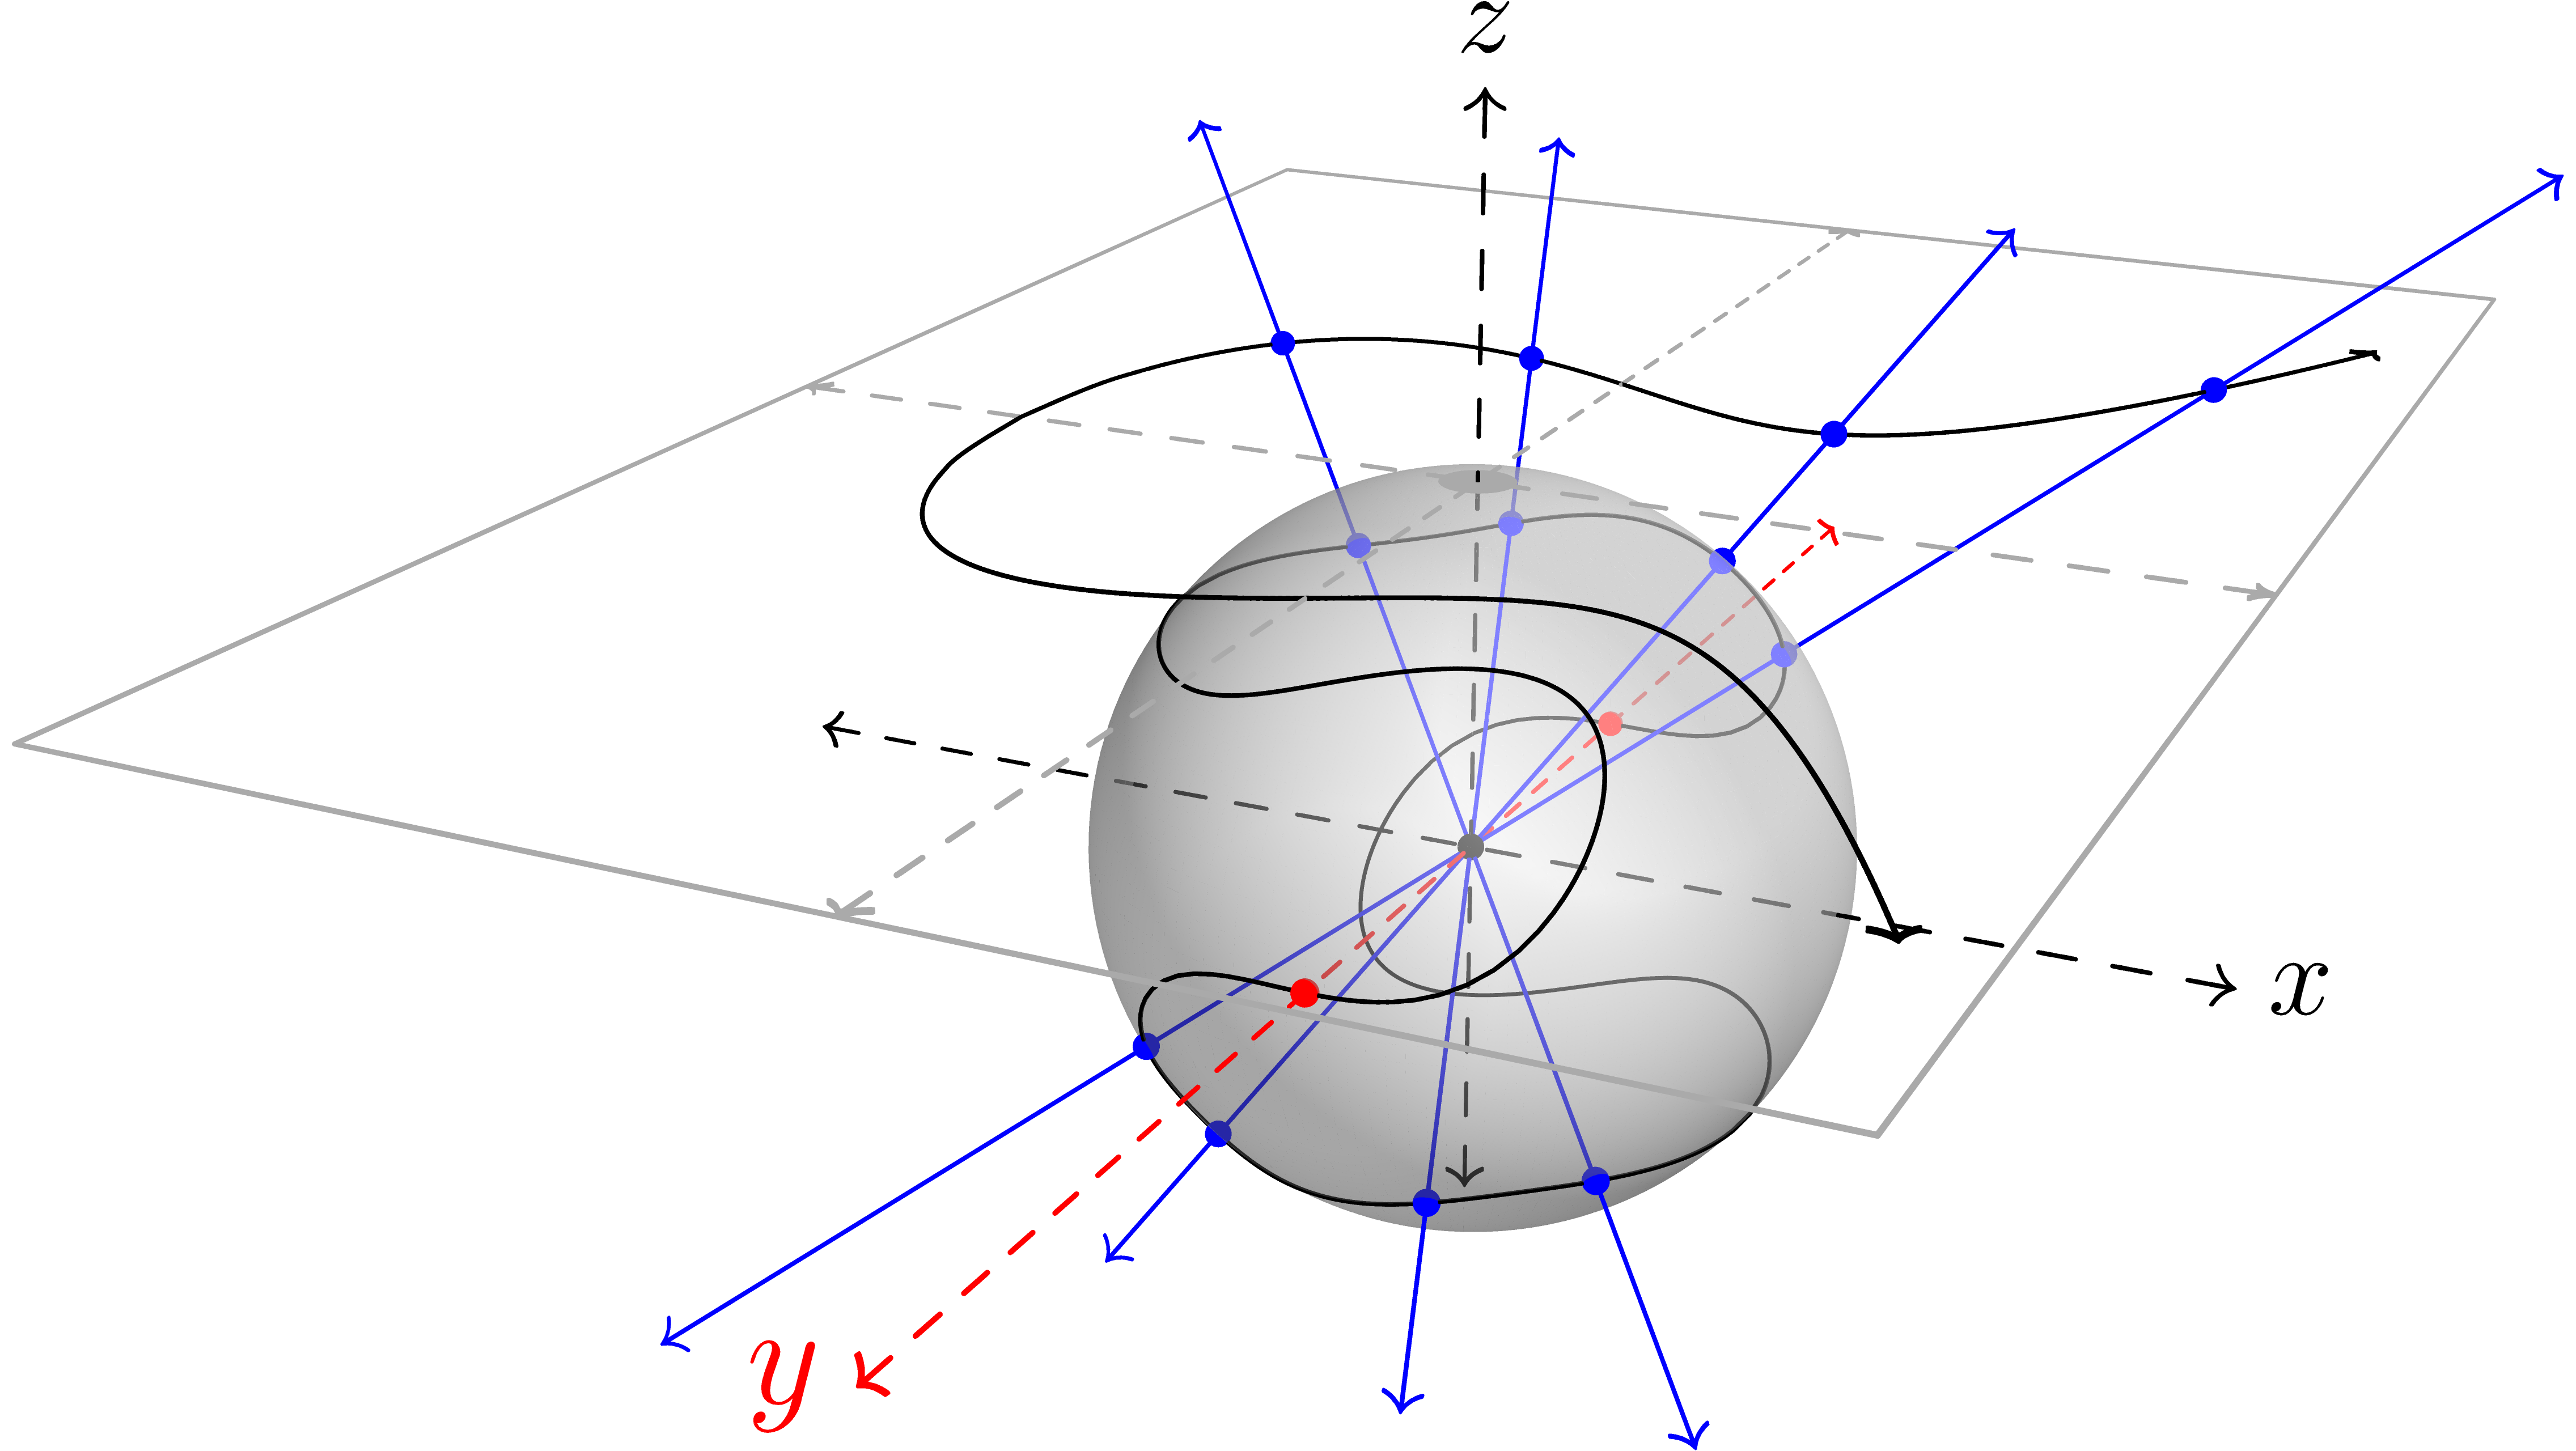
\includegraphics[height=0.57\textwidth]{ell-curve-projective.png}
  \end{figure}
\end{frame}

\begin{frame}
  \frametitle{zusätzliche Additionsregeln}
  \begin{definition}
    Seien $P = (x_p, y_p)$ und $Q =(x_q, y_q)$ zwei verschiedene Punkte auf der
    elliptischen Kurve $E$ mit $x_p = x_q$ (dann muss $y_q = -y_p$),
    oder sei $P = Q$ und $y_p = 0$.
    Sei $\mathcal{O}$ der Punkt im Unendlichen. Wir definieren:

    $$ P \oplus Q = \mathcal{O} $$
  \end{definition}
  \begin{Theorem}
    Mit dieser Erweiterung von \eqref{ec:add} für die Addition von Punkten einer
    elliptischen Kurve $E$ wird $(E, \oplus)$ zu einer {\bf Gruppe}.
  \end{Theorem}
\end{frame}

% ----------------------

\section{Endliche Körper}

\begin{frame}
  \frametitle{Körper}
  \begin{definition}
    Eine Menge in der die vier Grundrechenarten $+, -, *, /$ definiert sind,
    und die dafür üblichen Regeln gelten, nennt man {\bf Körper}
    (engl. {\bf field}).
  \end{definition}

  \pause
  Beispiele für Körper sind die reellen Zahlen $\R$, die rationalen
  Zahlen $\Q$ und die komplexen Zahlen $\mathbb{C}$.

  \pause
  \begin{folgerung}
    Sei K ein Körper, seien $a, b \in K$ mit $a \ne 0$ und $b \ne 0$.
    Dann gilt: $a * b \ne 0$.
  \end{folgerung}
\end{frame}

\begin{frame}
  \frametitle{Äquivalenzklassen mod N}
  \begin{definition}
    Sei $N \in \N, N > 1$. Zwei ganze Zahlen $a$ und $b$ heißen
    \emph{äquivalent modulo N}, geschrieben $a \equiv b \pmod N$, wenn
    $$ \exists m \in \Z: a-b = mN $$
  \end{definition}

  \begin{lemma}
    Sei $N \in \N, N > 1$, seien $a_1, a_2, b_1, b_2 \in \Z$,
    mit $a_1 \equiv a_2 \pmod N$ und $b_1 \equiv b_2 \pmod N$  dann gilt:
    \begin{equation}
      \begin{split}
        \label{op:mod}
        a_1 + b_1 & \equiv  a_2 + b_2 \pmod N \\
        a_1 \cdot b_1 & \equiv  a_2 \cdot b_2 \pmod N
      \end{split}
    \end{equation}
  \end{lemma}
\end{frame}

\begin{frame}
  \frametitle{Primkörper}

  $N$ beliebig? Nein:

  \begin{lemma}
  Sei $N$ eine zusammengesetzte Zahl, dann ist die Menge der
  Äquivalenzklassen $mod\ N$ kein Körper.
  \end{lemma}
  \begin{proof}
    N zusammengesetzt heißt, es gibt $n_1, n_2 \in \N$ mit $n_1 < N$
    und $n_2 < N$, so dass $n_1 n_2 = N$. Dann ist $n_1 \not\equiv 0$, und
    $n_2 \not\equiv 0$. Aber $n_1 n_2 \equiv 0$, im Widerspruch zur
    Körpereigenschaft oben.
  \end{proof}
  \begin{theorem}
    Sei $p$ eine Primzahl. Dann ist die Menge der Äquivalenzklassen $mod\ p$
    ein Körper: $\F_p$.
  \end{theorem}
\end{frame}

\begin{frame}
  \frametitle{Primkörper, Division}
  Um $\frac{a}{b}$ zu berechnen reicht es $\frac 1 b$ zu finden, also eine Zahl
  $b'$, so daß $b * b' \equiv 1 \pmod p$, bzw. zwei Zahlen $m$ und
  $b' \in \Z$, so dass $m * p + b' * b = 1$.
  \begin{beispiel}
    Sei $p = 37$, $b = 10$, wir suchen $b' \in \{0 \ldots 36\}$ und
    $m \in \Z$ mit $m * 37 + b' * 10 = 1$
  \end{beispiel}
\end{frame}

\begin{frame}
  \frametitle{Primkörper, Beispiel Division}
  \vspace*{-1cm}
  \begin{eqnarray}
    1 * 37 + 0 * 10 = 37  \label{ex:1} \\
    0 * 37 + 1 * 10 = 10  \label{ex:2}
  \end{eqnarray}
  $37 - 3 * 10 = 7$, add \eqref{ex:1} and $-3 * \eqref{ex:2}$
  \begin{eqnarray}
    1 *37 + (-3) * 10 = 7 \label{ex:3}
  \end{eqnarray}
  $10 - 1 * 7 = 3$, add \eqref{ex:2} and $-1 * \eqref{ex:3}$
  \begin{eqnarray}
    (-1) * 37 + 4 * 10 = 3 \label{ex:4}
  \end{eqnarray}
  $7 - 2*3 = 1$, add \eqref{ex:3} and $-2 * \eqref{ex:4}$
  \begin{eqnarray}
    (-3) * 37 + (-11) * 10 = 1
  \end{eqnarray}
  $\Rightarrow$ Inverse von 10 ist -11 bzw 26.
\end{frame}

\begin{frame}
  \frametitle{Elliptische Kurve über endlichem Körper}
  Anschaulichkeit leidet ein wenig:
  \begin{figure}
    \includegraphics[height=0.6\textwidth]{finplot.png}
  \end{figure}
\end{frame}
\begin{frame}
  \frametitle{Bemerkungen}
  Gibt es Kurven die genügend viele Punkte haben? Ja:
  \begin{theorem}[Hasse-Schranke]
    Sei E eine elliptische Kurve über $\F_p$. Sei $N$ die Anzahl der Punkte
    auf E, dann gilt:
    \begin{equation}
      \| N - p - 1 \| \le \sqrt{p}
    \end{equation}
  \end{theorem}
  In der Praxis werden momentan im Wesentlichen vier Kurven über vier
  verschiedenen Primkörpern benutzt, die Primzahlen haben dabei 76, 117 und
  156 Dezimalstellen.
\end{frame}

% ----------------------

\section{Diffie-Hellmann Schlüsselaustausch}

\begin{frame}
  Elliptische Kurven Diffie-Hellman
  \begin{itemize}
  \item Kein Signatur- oder Verschlüsselungsverfahren, sondern ein
    Schlüsselaustauschprotokoll
  \item Vorher festlegen: Endlicher Körper $\F_p$, elliptische Kurve E, über
    $\F_p$, also die Parameter $a$, $b$ der Weierstraß-Normalform, Basispunkt
    $P = (x_p, y_p)$.
  \item Am Schluss besitzen Alice und Bob denselben gemeinsamen Schlüssel.
  \end{itemize}
\end{frame}

\begin{frame}
  \frametitle{Diffie Hellman Schlüsselaustausch}
  \begin{equation*}
    \begin{CD}
      {\hbox to 0pt{\hss $s_A \in \N$ }}\text{\LARGE A}
      @. \text
      {\LARGE B}{\hbox to 0pt{ $s_B \in \N$\hss}} \\
      \text{\LARGE A}
      @>\ \overbrace{P + \ldots + P}^{s_A-mal} = P_A\ >>
      \text{\LARGE B} \\
      \text{\LARGE A}
      @<\ P_B = \overbrace{P + \ldots + P}^{s_B-mal}\ <<
      \text{\LARGE B} \\
      {\hbox to 0pt{\hss $P_S = \overbrace{P_B + \ldots + P_B}^{s_A-mal}$ }}
      \text{\LARGE A}
      @.
      \text{\LARGE B}
      {\hbox to 0pt{ $P_S = \overbrace{P_A + \ldots + P_A}^{s_B-mal}$\hss}}
    \end{CD}
  \end{equation*}
\end{frame}

\begin{frame}
  \frametitle{Zusammenfassung}
  \vspace*{-1cm}
  Was hatten wir?
  \begin{itemize}
  \item Ein Kurve, wahlweise in Fisch- oder Knubbelform.
  \item Eine geometrische Operation $\oplus$ auf der Kurve, die zu zwei
    Punkten einen dritten bestimmt.
  \item Ein Ausflug in die dritte Dimension, der der Kurve einen extra Punkt
    hinzufügt. Nun ist $\oplus$ eine Addition.
  \item Ein Ausflug in endliche Körper, danach kann ein Computer mit diesen
    Punkten rechnen.
  \item Ein Protokoll, wie man sich mit diesen Punkten über einen öffentlichen
    Kanal ein gemeinsames Geheimnis erzeugt.
  \end{itemize}
\end{frame}

\begin{frame}
  \begin{center}
    \Large Danke für Eure Aufmerksamkeit
  \end{center}
\end{frame}

\end{document}
